% ------------------------------------------------------------------
%  Physics 1: Mechanics -- Week 1 homework review
%  Compile with:  tectonic week1-review.tex
% ------------------------------------------------------------------
\documentclass[11pt]{article}

\usepackage[T1]{fontenc}
\usepackage[utf8]{inputenc}
\usepackage{lmodern}
\usepackage[letterpaper,top=0.8in,bottom=0.8in,left=1.0in,right=1.0in]{geometry}
\usepackage{amsmath,amssymb}
\usepackage{siunitx}
\usepackage{tikz}
\usetikzlibrary{arrows.meta,calc}
\usepackage[most]{tcolorbox}
\usepackage{booktabs}
\usepackage{enumitem}
\usepackage{microtype}
\usepackage{fancyhdr}
\usepackage[hidelinks]{hyperref}
\usepackage{titlesec}

\sisetup{per-mode=symbol,separate-uncertainty=true}
\newcommand{\dd}{\mathrm{d}}

\pagestyle{fancy}
\fancyhf{}
\fancyhead[L]{\small Physics 1: Mechanics \textperiodcentered\ Week 1 review}
\fancyhead[R]{\small\thepage}
\renewcommand{\headrulewidth}{0.4pt}

\definecolor{teal}{RGB}{0,140,150}
\definecolor{tealpale}{RGB}{232,246,247}
\definecolor{sand}{RGB}{252,245,230}
\definecolor{sanddark}{RGB}{190,140,60}
\definecolor{plum}{RGB}{110,60,130}
\definecolor{plumpale}{RGB}{243,236,247}
\definecolor{slate}{RGB}{70,80,95}
\definecolor{slatepale}{RGB}{240,242,245}
\definecolor{wrongcol}{RGB}{170,40,40}
\definecolor{wrongpale}{RGB}{252,238,238}
\definecolor{rightcol}{RGB}{25,120,70}
\definecolor{rightpale}{RGB}{233,246,238}

\titleformat{\section}{\large\bfseries\color{slate}}{\thesection}{0.7em}{}
\titleformat{\subsection}{\bfseries}{\thesubsection}{0.6em}{}

\newtcolorbox{point}[1][Knowledge point]{%
  enhanced,breakable,colback=sand,colframe=sanddark,fonttitle=\bfseries,
  title={#1},sharp corners,boxrule=0.8pt,left=3mm,right=3mm,
  before skip=10pt,after skip=10pt}

\newtcolorbox{whatwrong}[1][What went wrong]{%
  enhanced,breakable,colback=wrongpale,colframe=wrongcol,fonttitle=\bfseries,
  coltitle=white,title={#1},sharp corners,boxrule=0.7pt,left=3mm,right=3mm,
  before skip=8pt,after skip=8pt}

\newtcolorbox{whatright}[1][What you got right]{%
  enhanced,breakable,colback=rightpale,colframe=rightcol,fonttitle=\bfseries,
  coltitle=white,title={#1},sharp corners,boxrule=0.7pt,left=3mm,right=3mm,
  before skip=8pt,after skip=8pt}

\newtcolorbox{habit}[1][Habit]{%
  enhanced,breakable,colback=tealpale,colframe=teal,fonttitle=\bfseries,
  coltitle=white,title={#1},sharp corners,boxrule=0.7pt,left=3mm,right=3mm,
  before skip=8pt,after skip=8pt}

\setlist[enumerate]{itemsep=3pt,topsep=3pt}
\setlist[itemize]{itemsep=3pt,topsep=3pt}

\begin{document}

\begin{center}
{\LARGE\bfseries Week 1 Homework Review}\\[4pt]
{\large Scholars High School Physics 1: Mechanics}\\[6pt]
{\small Writing problem: Technical 5.5\,/\,7, Style 1\,/\,1 \quad\textperiodcentered\quad
Challenge problems: 10\,/\,10, one retry}
\end{center}

\vspace{4pt}

\begin{point}[The headline]
Your physics was right. Every conceptual step in the writing problem was correct, and
the grader said so. The marks came off for \emph{bookkeeping}: an assumed scale, an
unchecked formula, and a missing sanity check. That is good news --- these are habits,
and habits are far quicker to fix than understanding.
\end{point}

\section{What you got right}

\begin{whatright}
\begin{itemize}
  \item \textbf{(a) Direction is unknowable.} A dot diagram records positions, not the
        order they were visited. You said so and explained why. Full credit.
  \item \textbf{(b) The speed increases.} You compared distances covered in equal time
        intervals --- exactly the right reading of a dot diagram --- and drew the right
        conclusion.
  \item \textbf{(d) The centred-interval technique.} To estimate the speed \emph{at} the
        second-to-last dot you used the dots on \emph{either side} of it rather than one
        adjacent gap. That is the correct method, and a lot of students get it wrong.
        The grader specifically approved the choice of dots and the elapsed time.
\end{itemize}
\end{whatright}

\section{What went wrong}

\subsection*{1. You invented a scale instead of deriving one}

This is the big one, and it caused both numerical errors.

You read the dot positions off the drawing as
\[
0,\; 1,\; 4,\; 9,\; 16,\; 25,\; 36
\]
and then wrote \emph{``given that position $n$ and position $n+1$ are one meter apart.''}
Those numbers are real, but they are \textbf{coordinates of the drawing}, not metres.
Nothing in the problem said one coordinate unit was a metre --- that was an assumption,
and it was wrong by a factor of nearly three hundred.

\begin{whatwrong}[Where the metres had to come from]
The diagram was printed at a stated scale of $1:1$, so a ruler laid on it measures real
distances. The last gap spans $36 - 25 = 11$ coordinate units and measures
\SI{3.9}{\centi\metre}. That one measurement fixes everything:
\[
1\ \text{coordinate unit} = \frac{\SI{3.9}{\centi\metre}}{11} = \SI{0.35}{\centi\metre}
= \SI{3.5}{\milli\metre}.
\]
\end{whatwrong}

With the scale in hand, the two answers come out as follows.

\begin{center}
\renewcommand{\arraystretch}{1.3}
\setlength{\tabcolsep}{5pt}
\begin{tabular}{@{}lll@{}}
\toprule
 & \textbf{your answer} & \textbf{correct answer} \\
\midrule
(c) average speed
  & $\dfrac{36}{6} = \SI{6}{\metre\per\second}$
  & $\dfrac{36 \times \SI{0.35}{\centi\metre}}{\SI{6}{\second}}
     = \SI{2.1}{\centi\metre\per\second}$ \\[10pt]
(d) instantaneous speed
  & $\dfrac{36-16}{7-5} = \SI{10}{\metre\per\second}$
  & $\dfrac{20 \times \SI{0.35}{\centi\metre}}{\SI{2}{\second}}
     = \SI{3.5}{\centi\metre\per\second}$ \\[6pt]
\bottomrule
\end{tabular}
\end{center}

\medskip
Notice that both answers are too large by the \emph{same} factor of \num{282}. That is
the signature of one bad conversion, not two separate mistakes --- and it is why fixing
the single habit fixes both parts.

\subsection*{2. You wrote the formula upside down}

In part (b) you wrote:

\begin{center}
\textcolor{wrongcol}{``\,distance $=$ speed\,/\,time\,''}
\qquad instead of \qquad
\textcolor{rightcol}{distance $=$ average speed $\times$ time}
\end{center}

The calculations that followed used $d/t$ correctly, so the wrong formula never actually
got used --- which is precisely why it survived to the page. A reader can only judge what
you wrote, and the next time you reach for that formula on a problem where the right
answer is not obvious, you will follow the words.

\begin{habit}[Check a rearrangement with units, every time]
Substitute units for quantities and see whether both sides match. It takes five seconds
and needs no physics:
\[
\frac{\si{\metre\per\second}}{\si{\second}} = \si{\metre\per\second\squared}
\quad\text{(an acceleration --- not a distance)},
\qquad
\si{\metre\per\second} \times \si{\second} = \si{\metre} \quad\text{\checkmark}
\]
\end{habit}

\subsection*{3. No sanity check}

\SI{6}{\metre\per\second} is a fast run --- roughly \SI{22}{\kilo\metre\per\hour}. The
diagram is a few centimetres across and covers six seconds. Those two facts cannot both
be true, and noticing the clash costs nothing.

\begin{center}
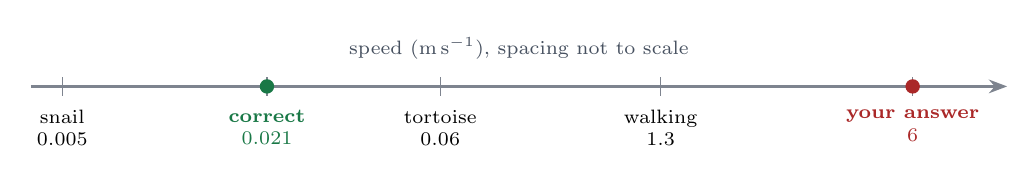
\begin{tikzpicture}[x=1cm,y=1cm]
  \draw[->,>=Stealth,slate!70,thick] (0,0) -- (12.4,0);
  \foreach \x/\lab in {0.4/{\SI{0.005}{}},3.0/{\SI{0.021}{}},5.2/{\SI{0.03}{}},8.0/{\SI{1.3}{}},11.2/{\SI{6}{}}}{
    \draw[slate!70] (\x,-0.12) -- (\x,0.12);}
  \node[font=\scriptsize,anchor=north,align=center] at (0.4,-0.18) {snail\\ \SI{0.005}{}};
  \node[font=\scriptsize,anchor=north,align=center,rightcol] at (3.0,-0.18) {\textbf{correct}\\ \textbf{\SI{0.021}{}}};
  \node[font=\scriptsize,anchor=north,align=center] at (5.2,-0.18) {tortoise\\ \SI{0.06}{}};
  \node[font=\scriptsize,anchor=north,align=center] at (8.0,-0.18) {walking\\ \SI{1.3}{}};
  \node[font=\scriptsize,anchor=north,align=center,wrongcol] at (11.2,-0.18) {\textbf{your answer}\\ \textbf{\SI{6}{}}};
  \fill[rightcol] (3.0,0) circle (2.6pt);
  \fill[wrongcol] (11.2,0) circle (2.6pt);
  \node[font=\scriptsize,anchor=south,slate] at (6.2,0.22) {speed (\si{\metre\per\second}), spacing not to scale};
\end{tikzpicture}
\end{center}

\subsection*{4. A phrasing slip}

You wrote \emph{``the instantaneous speed occurs between the 5th dot and the 7th dot.''}
It does not occur between anything. Instantaneous speed is the speed \textbf{at one
instant}; what you computed was an average over the surrounding interval, which
\textbf{estimates} the instantaneous speed \textbf{at the middle dot}. The method was
right --- only the sentence was loose. Say it as:

\begin{quote}
``The average speed from dot 5 to dot 7 estimates the instantaneous speed \emph{at} dot 6,
because the interval is centred on that dot.''
\end{quote}

\section{The same pattern showed up again}

Week 2, Problem 2 (notation matching, 5\,/\,7 after a retry): your first attempt swapped
$v$ and $v_x$. Not a concept error --- a subscript error. Same family as everything above.

\begin{center}
\renewcommand{\arraystretch}{1.3}
\begin{tabular}{@{}llll@{}}
\toprule
symbol & name & sign & read it as \\
\midrule
$x$      & coordinate along $x$   & either        & ``where it is, relative to the origin'' \\
$\Delta x$ & displacement along $x$ & either        & ``how far and which way it moved'' \\
$v_x$    & velocity along $x$     & either        & ``how fast and which way it is going'' \\
$v$      & speed                  & never negative & ``how fast it is going'' \\
\bottomrule
\end{tabular}
\end{center}

\medskip
\textbf{The rule in one line:} a subscript names an axis and keeps the sign; a bare $v$
means speed and never carries one.

\section{The knowledge point}

\begin{point}[Numbers read off a diagram are in the diagram's units]
\textbf{Read $\rightarrow$ Convert $\rightarrow$ Divide $\rightarrow$ Check.}
\begin{enumerate}
  \item \textbf{Read} the positions in the diagram's own units, and \emph{name} them:
        write ``\num{36} squares,'' never a bare ``\num{36}.'' A number with its unit
        attached makes the missing conversion visible, because \si{\text{squares}\per\second}
        is not a speed.
  \item \textbf{Convert} using a scale you \emph{measured or were given}: one length in
        the diagram whose true size you know. If you cannot point at that measurement,
        you assumed a scale rather than found one.
  \item \textbf{Divide} by the elapsed time --- and count intervals, not dots.
  \item \textbf{Check} by converting into units you have a feel for before writing the
        answer down.
\end{enumerate}
\end{point}

\begin{habit}[Three questions, thirty seconds, before you submit]
\begin{enumerate}
  \item \emph{Have I named the units at every step?} A bare number is an invitation to
        divide it by seconds and call the result \si{\metre\per\second}.
  \item \emph{Where did my metres come from?} Trace them back to a real ruler
        measurement or a given scale. No trace, no metres.
  \item \emph{Does the size make sense?} Convert into something you can picture and
        compare it with a thing you know.
\end{enumerate}
\end{habit}

\section{Where this now lives in the book}

Chapter 1 of \emph{Physics 1: Mechanics} was rewritten around these four points
(\num{46} $\rightarrow$ \num{53} pages). \textbf{\S1.3, ``Grid units are not metres''}
is new: the three-step rule, a dot diagram on a grid with the ruler measurement marked,
a worked example on fresh numbers, and a modelling note, ``Three habits that catch this
error.'' \textbf{\S1.4} adds ``Check a rearrangement with its units''; \textbf{\S1.5} the
centred estimate $v_n \approx (x_{n+1}-x_{n-1})/2\tau$ and the phrasing point;
\textbf{\S1.9} the symbols table above. Plus \num{8} new exercises and \num{2} new
check-your-understanding boxes, all answered.

\bigskip
\begin{center}
\small\itshape
Sources: your graded Week 1 homework and Week 2 Problem 2, AoPS course 4926.
\end{center}

\end{document}
